\documentclass{article}

\usepackage{polski}
\usepackage[utf8]{inputenc}
\usepackage{booktabs}
\usepackage{biblatex}
\usepackage{subfigure}
\usepackage{graphicx}
\usepackage{float}
\usepackage{geometry}
\usepackage{listings}

 \usepackage[table,xcdraw]{xcolor}

\geometry{
	a4paper,
	total={170mm,257mm},
	left=50mm,
	right=50mm,
	top=45mm,
	bottom = 45mm
}
\usepackage{tabularx}


\begin{document}
	\newgeometry{tmargin=4cm, bmargin=4cm, lmargin=3cm, rmargin=3cm}
	
	\begin{titlepage}
		\center
		\newcommand{\HRule}{\rule{\linewidth}{0.6mm}}
		
		\textsc{\LARGE Politechnika Wrocławska}\\[1.5cm]
		\textsc{\Large Laboratorium}\\[0.5cm] 
		\textsc{\large Inteligencja Obliczeniowa i jej Zastosowania}\\[0.7cm] 

		\HRule \\[0.4cm]
		{ \huge \bfseries Algorytmy ewolucyjne i hybrydowe}\\[0.4cm]
		\HRule \\[1.5cm]
		
		\begin{minipage}{0.4\textwidth}
			\begin{flushleft} \large
				\emph{Authors:}\\
				Rafał \textsc{Pieniążek}\\
                Jakub \textsc{Pomykała}
			\end{flushleft}
		\end{minipage}
		~
		\begin{minipage}{0.4\textwidth}
			\begin{flushright} \large
				\emph{Supervisor:} \\
				prof. dr inż. Olgierd \textsc{Unold} 
			\end{flushright}
		\end{minipage}\\[4cm]

		{\large \today}\\[3cm]
		
		\vfill
		
	\end{titlepage}
\tableofcontents
\newpage
\listoffigures
\newpage
\section{Wstęp}
	Celem laboratorium było przeprowadzenie optymalizacji globalnej dla wybranych funkcji z pakietu globalOptTests.
    

\section{Zastosowany algorytm optymalizacji}

W laboratorium zastosowano algorytmy genetyczne będące klasą algorytmów ewolucyjnych.
Algorytmy ewolucyjne stanowią kierunek sztucznej inteligencji, która wykorzystuje i symuluje ewolucję biologiczną. Wszystkie algorytmy tej klasy symulują podstawowe zachowania w teorii ewolucji biologicznej - procesy selekcji, mutacji i reprodukcji. Zachowanie jednostek zależy od środowiska. Zbiór jednostek nazywa się populacją. Taka populacja ewoluuje zgodnie z regułami selekcji zgodnie z funkcją celu przypisaną do środowiska. Propagowane do kolejnych pokoleń są tylko najbardziej dopasowane osobniki.


\subsection{Modyfikowane parametry}

W celu badania wpływu zmiennych na zachowanie algorytmu genetycznego modyfikowano następujące parametry:

\begin{itemize}
\item \textbf{elitarność} - Procentowa wartość populacji, która zostaje przeniesiona do następnego pokolenia bez zmian. Niezerowa wartość gwarantuje, że jakość rozwiązania nie zmniejszy się z pokolenia na pokolenie.

\item \textbf{mutacja} - Przypadkowa zmiana genomu w algorytmie genetycznym, analogicznie do mutacji biologicznej.

\item \textbf{krzyżowanie} -  Połączenie niektórych (wybranych losowo) genotypów w jeden. Kojarzenie ma sprawić, że potomek dwóch osobników rodzicielskich ma zespół cech, który jest kombinacją ich cech (może się zdarzyć, że tych najlepszych).

\item \textbf{liczba iteracji} - Ilość pokoleń  
\item \textbf{rozmiar populacji} - Ilość osobników w jednym pokoleniu.
\end{itemize}


\begin{table}[!htbp]
\centering
\caption{Wartości modyfikowanych parametrów}
\label{my-label}
\begin{tabular}{|l|l|}
\hline
\rowcolor[HTML]{C0C0C0} 
\textbf{Parametr}      & \textbf{Wartości}      \\ \hline
populacja              & 50, 100, 150, 200, 250 \\ \hline
liczba iteracji        & 50, 100, 150, 200, 250 \\ \hline
p. krzyżowania         & 0, 0.25, 0.5, 0.75, 1  \\ \hline
p. mutacji             & 0, 0.25, 0.5, 0.75, 1  \\ \hline
p. populacji elitarnej & 0, 0.25, 0.5, 0.75, 1  \\ \hline
\end{tabular}
\end{table}


\subsection{Zastosowane narzędzia implementacji}

\subsubsection{Język R}
R jest językiem programowania i środowiskiem programistycznym, używanym głównie do obliczeń statystycznych i wizualizacji danych, do sztucznej inteligencji a także do ekonomii i innych zagadnień wykorzystujących obliczenia numeryczne. Został stworzony przez Rossa Ihakę i Roberta Gentlemana na Uniwersytecie w Auckland w Nowej Zelandii. 


\subsubsection{Pakiet GA}

Pakiet GA zawiera zestaw funkcji ogólnego przeznaczenia do optymalizacji z wykorzystaniem algorytmów genetycznych. Dostępnych jest kilka operatorów genetycznych, których można łączyć w celu zbadania najlepszych ustawień dla bieżącego zadania.


\subsubsection{Pakiet globalOpts}
Pakiet zawierający implementację funkcji przydatnych do przeprowadzania testów wydajnościowych algorytmów optymalizacji globalnej.


\clearpage
\section{Funkcja Shuberta}
	\subsection{Wzór analityczny}
	   \begin{figure}[!htbp]
    \centering
    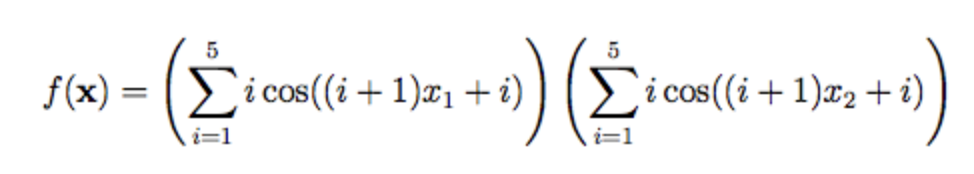
\includegraphics[width=0.6\textwidth]{inc/wzory/schubert}
     \caption{Wzór analityczny funkcji Schuberta}
    \end{figure}
    
    
 
    
    
    \subsection{Wykres w ustalonym przedziale zmiennych}
    
    \begin{figure}[!h]
    \centering
    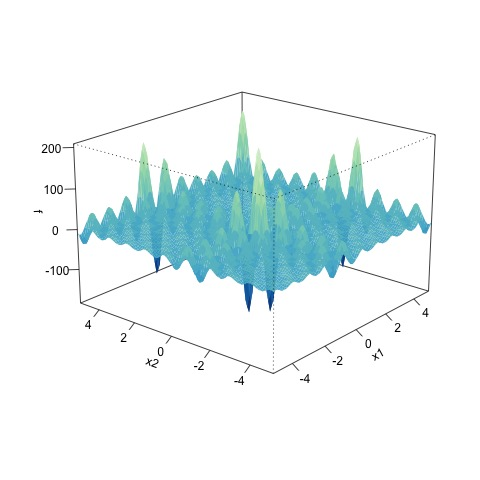
\includegraphics[width=0.6\textwidth]{inc/wykresyfunkcji/schubert}
     \caption{Wykres  funkcji Schuberta}
    \end{figure}
    
    \subsection{Ekstremum globalne}
    
       \begin{figure}[!h]
    \centering
    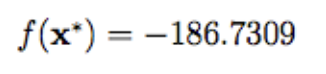
\includegraphics[width=0.3\textwidth]{inc/wzory/schubert-global-minimum}
     \caption{Minimum globalne dla funkcji Schuberta}
    \end{figure}
    
       \begin{figure}[!h]
    \centering
    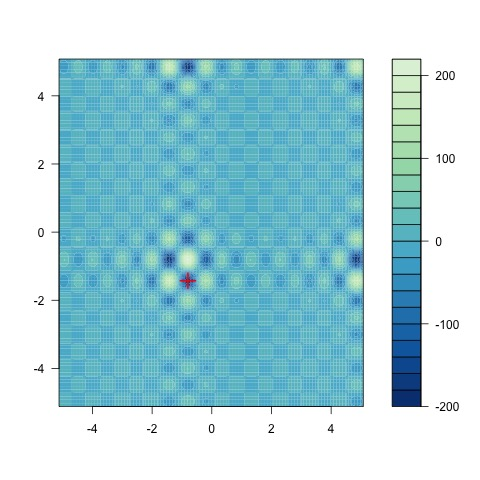
\includegraphics[width=0.7\textwidth]{inc/wykresyfunkcji/schubert-global-minimum}
     \caption{Minimum globalne dla funkcji Schuberta}
    \end{figure}
    
    \subsection{Optymalizacja poszukiwania ekstremum globalnego}

\subsubsection{Modyfikacja parametru elitarności}

W przypadku zwiększania wartości elitarności populacji średnie wartości odchyleń zmniejszają się. W przypadku większej elitarności algorytm szybciej znajduje optymalne rozwiązanie. Jeżeli elitarność populacji jest równa 1, to algorytm stochastycznie wylosował jeden zestaw rozwiązań, który z powodu braku ewolucji nie zbliżył się do rozwiązania optymalnego.


\begin{figure}[!htbp]
    \centering
\mbox{
\subfigure{
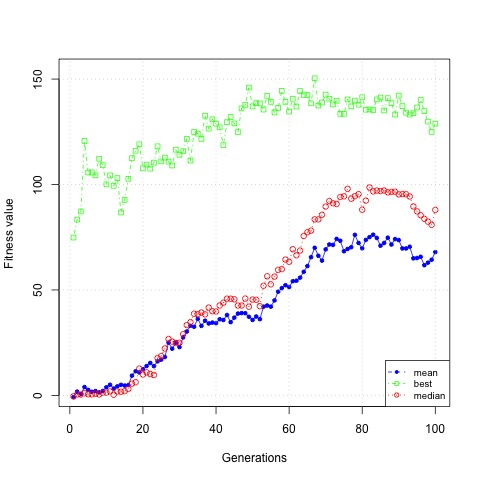
\includegraphics[width=3in]{{{inc/results/generations-Schubert-p050-i100-c0.80-m0.10-e0.00}}}\quad
}
\subfigure{
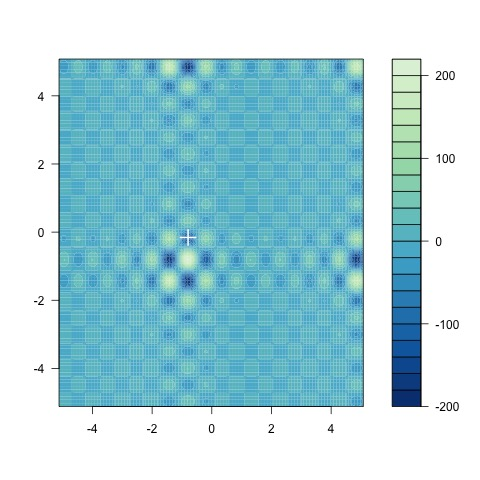
\includegraphics[width=3in]{{{inc/results/result-Schubert-p050-i100-c0.80-m0.10-e0.00}}}\quad
}
}
                 \caption{Test optymalizacji GA Schubert p50 i100 c0.8 m0.1 e0}
                 \end{figure}
\begin{figure}[!htbp]
    \centering
\mbox{
\subfigure{
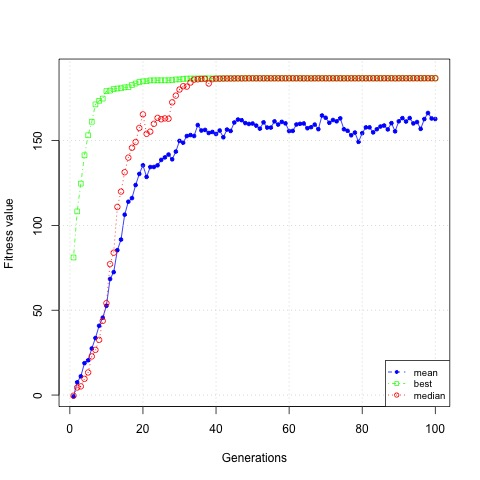
\includegraphics[width=3in]{{{inc/results/generations-Schubert-p050-i100-c0.80-m0.10-e0.25}}}\quad
}
\subfigure{
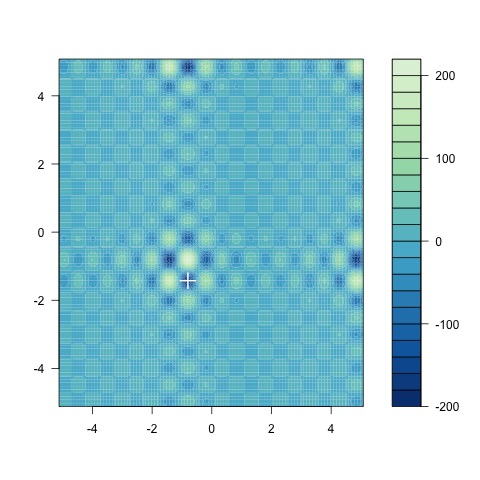
\includegraphics[width=3in]{{{inc/results/result-Schubert-p050-i100-c0.80-m0.10-e0.25}}}\quad
}
}
                 \caption{Test optymalizacji GA Schubert p50 i100 c0.8 m0.1 e0.25}
                 \end{figure}
\begin{figure}[!htbp]
    \centering
\mbox{
\subfigure{
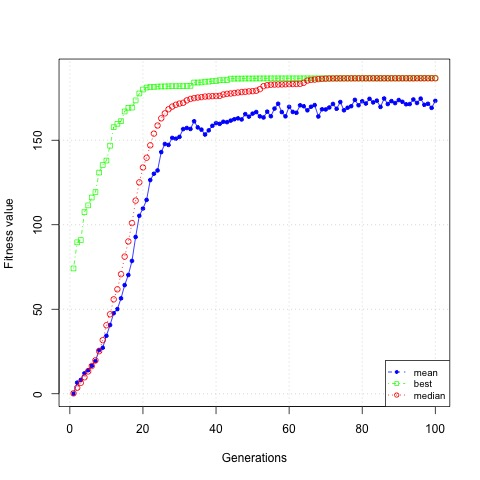
\includegraphics[width=3in]{{{inc/results/generations-Schubert-p050-i100-c0.80-m0.10-e0.50}}}\quad
}
\subfigure{
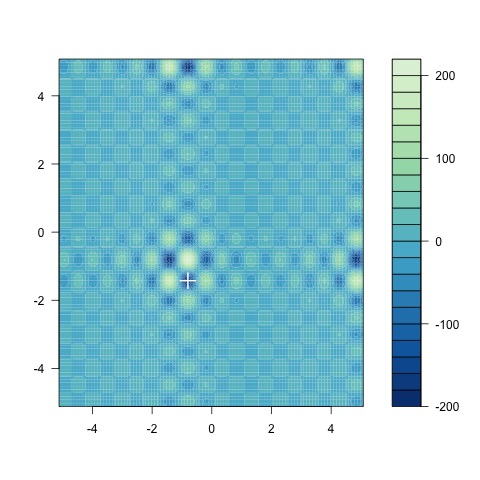
\includegraphics[width=3in]{{{inc/results/result-Schubert-p050-i100-c0.80-m0.10-e0.50}}}\quad
}
}
                 \caption{Test optymalizacji GA Schubert p50 i100 c0.8 m0.1 e0.5}
                 \end{figure}
\begin{figure}[!htbp]
    \centering
\mbox{
\subfigure{
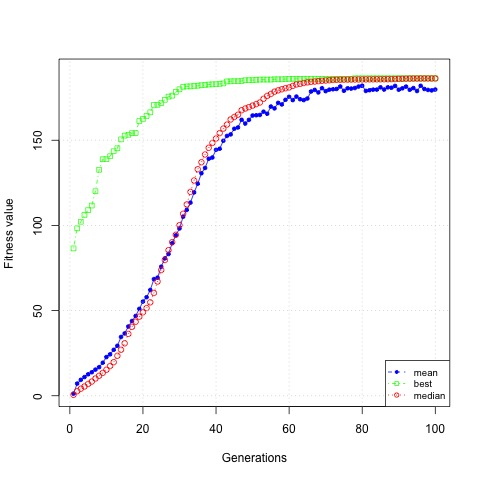
\includegraphics[width=3in]{{{inc/results/generations-Schubert-p050-i100-c0.80-m0.10-e0.75}}}\quad
}
\subfigure{
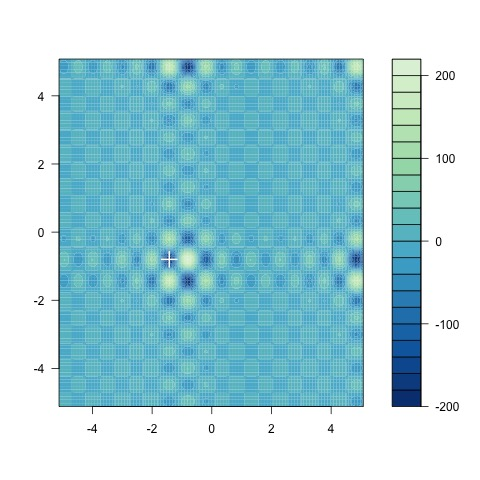
\includegraphics[width=3in]{{{inc/results/result-Schubert-p050-i100-c0.80-m0.10-e0.75}}}\quad
}
}
                 \caption{Test optymalizacji GA Schubert p50 i100 c0.8 m0.1 e0.75}
                 \end{figure}
\begin{figure}[!htbp]
    \centering
\mbox{
\subfigure{
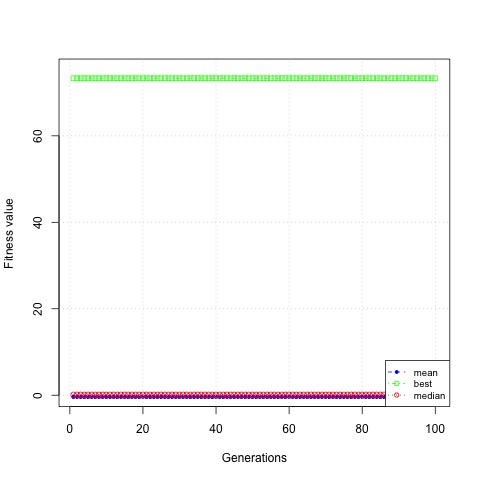
\includegraphics[width=3in]{{{inc/results/generations-Schubert-p050-i100-c0.80-m0.10-e1.00}}}\quad
}
\subfigure{
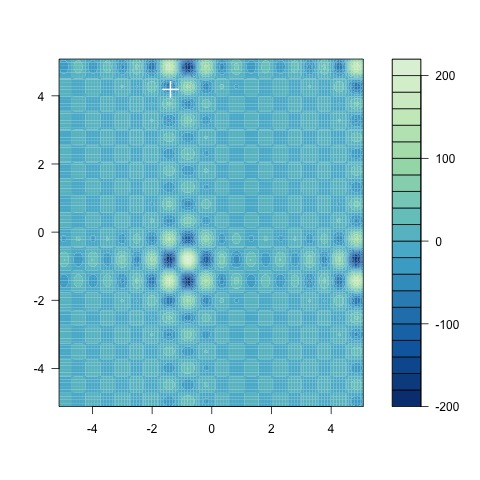
\includegraphics[width=3in]{{{inc/results/result-Schubert-p050-i100-c0.80-m0.10-e1.00}}}\quad
}
}
                 \caption{Test optymalizacji GA Schubert p50 i100 c0.8 m0.1 e1}
                 \end{figure}
\begin{figure}[!htbp]
\clearpage


\subsubsection{Modyfikacja parametru mutacji}

W przypadku zwiększania wartości mutacji zarówno średnia jak i mediana zmniejszają się. Algorytm zawsze znajduje po podobnej liczbie populacji rozwiązanie optymalne.

    \centering
\mbox{
\subfigure{
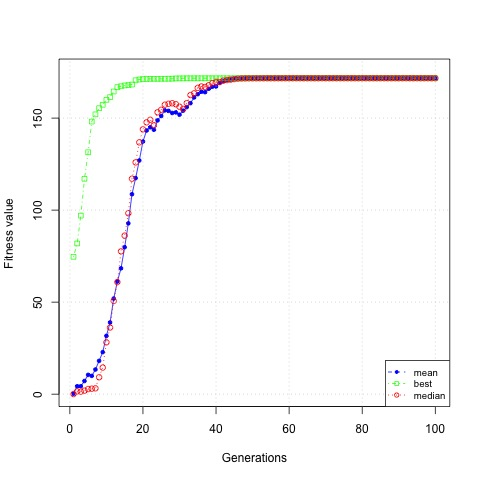
\includegraphics[width=3in]{{{inc/results/generations-Schubert-p050-i100-c0.80-m0.00-e0.05}}}\quad
}
\subfigure{
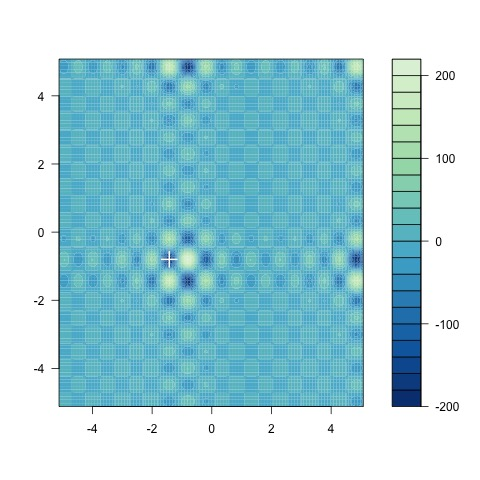
\includegraphics[width=3in]{{{inc/results/result-Schubert-p050-i100-c0.80-m0.00-e0.05}}}\quad
}
}
                 \caption{Test optymalizacji GA Schubert p50 i100 c0.8 m0 e0.05}
                 \end{figure}
\begin{figure}[!htbp]
    \centering
\mbox{
\subfigure{
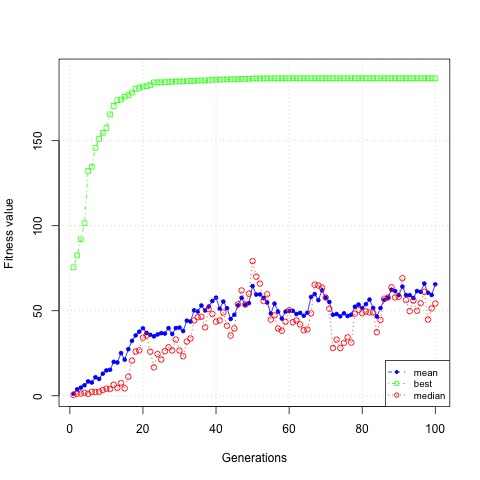
\includegraphics[width=3in]{{{inc/results/generations-Schubert-p050-i100-c0.80-m0.25-e0.05}}}\quad
}
\subfigure{
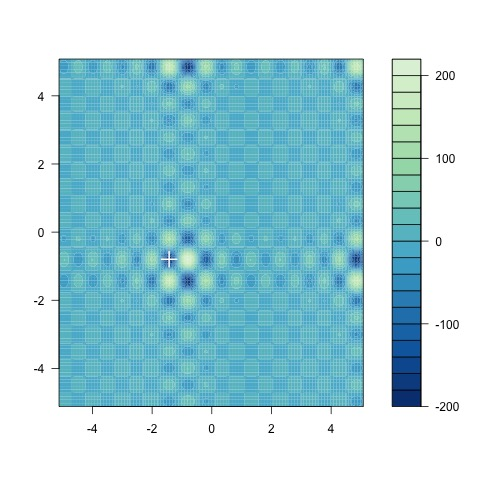
\includegraphics[width=3in]{{{inc/results/result-Schubert-p050-i100-c0.80-m0.25-e0.05}}}\quad
}
}
                 \caption{Test optymalizacji GA Schubert p50 i100 c0.8 m0.25 e0.05}
                 \end{figure}
\begin{figure}[!htbp]
    \centering
\mbox{
\subfigure{
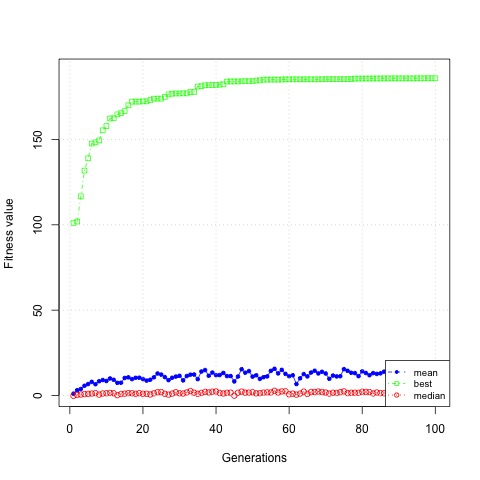
\includegraphics[width=3in]{{{inc/results/generations-Schubert-p050-i100-c0.80-m0.50-e0.05}}}\quad
}
\subfigure{
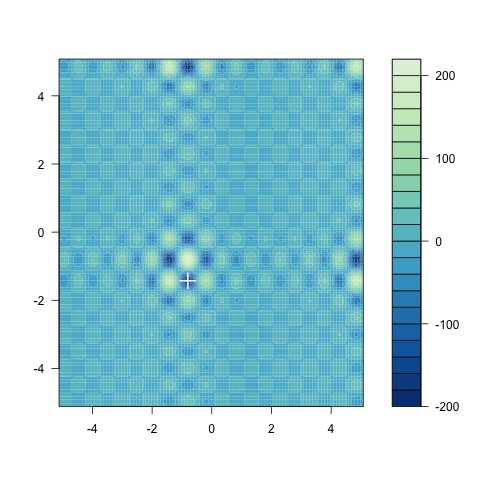
\includegraphics[width=3in]{{{inc/results/result-Schubert-p050-i100-c0.80-m0.50-e0.05}}}\quad
}
}
                 \caption{Test optymalizacji GA Schubert p50 i100 c0.8 m0.5 e0.05}
                 \end{figure}
\begin{figure}[!htbp]
    \centering
\mbox{
\subfigure{
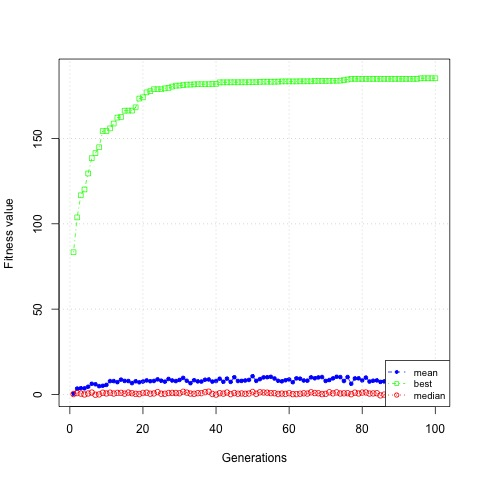
\includegraphics[width=3in]{{{inc/results/generations-Schubert-p050-i100-c0.80-m0.75-e0.05}}}\quad
}
\subfigure{
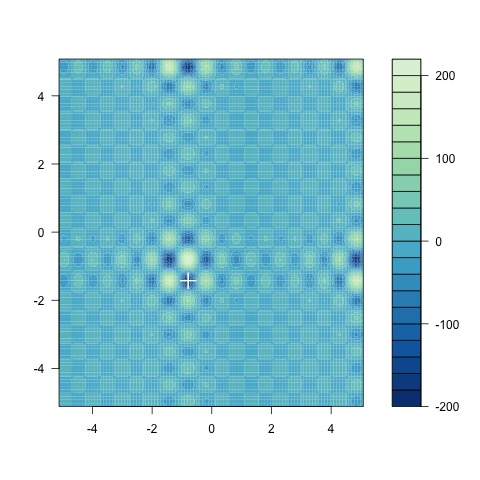
\includegraphics[width=3in]{{{inc/results/result-Schubert-p050-i100-c0.80-m0.75-e0.05}}}\quad
}
}
                 \caption{Test optymalizacji GA Schubert p50 i100 c0.8 m0.75 e0.05}
                 \end{figure}
\begin{figure}[!htbp]
    \centering
\mbox{
\subfigure{
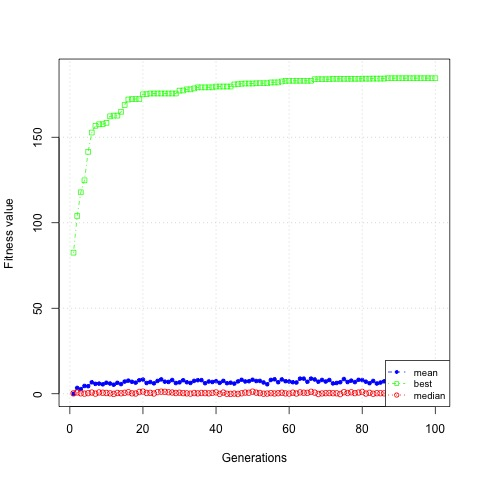
\includegraphics[width=3in]{{{inc/results/generations-Schubert-p050-i100-c0.80-m1.00-e0.05}}}\quad
}
\subfigure{
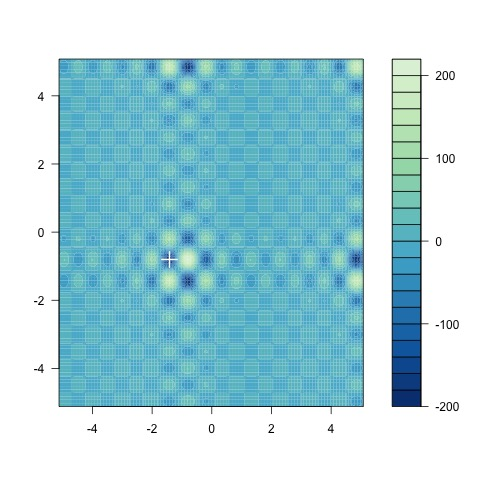
\includegraphics[width=3in]{{{inc/results/result-Schubert-p050-i100-c0.80-m1.00-e0.05}}}\quad
}
}
                 \caption{Test optymalizacji GA Schubert p50 i100 c0.8 m1 e0.05}
                 \end{figure}


                 
\clearpage
\subsubsection{Modyfikacja parametru krzyżowania}

W przypadku zwiększania parametru krzyżowania algorytm szybciej znajduje lokalne minimum, ale nie zawsze jest to ekstremum globalne. Wartości średniej i mediany pozostają na podobnym poziomie  niezależnie od parametrów.


\begin{figure}[!htbp]
    \centering
\mbox{
\subfigure{
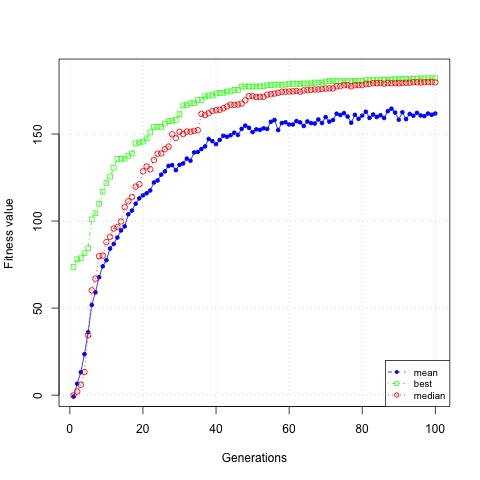
\includegraphics[width=3in]{{{inc/results/generations-Schubert-p050-i100-c0.00-m0.10-e0.05}}}\quad
}
\subfigure{
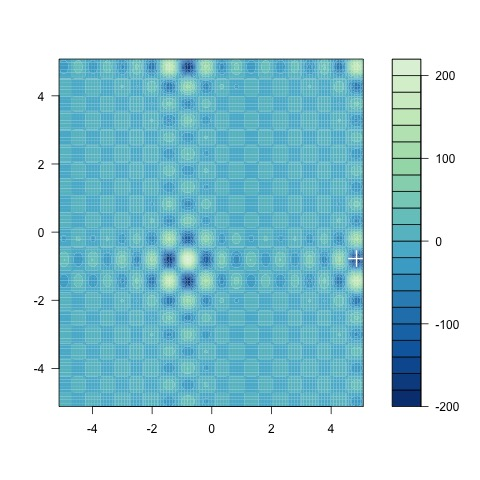
\includegraphics[width=3in]{{{inc/results/result-Schubert-p050-i100-c0.00-m0.10-e0.05}}}\quad
}
}
                 \caption{Test optymalizacji GA Schubert p50 i100 c0 m0.1 e0.05}
                 \end{figure}
\begin{figure}[!htbp]
    \centering
\mbox{
\subfigure{
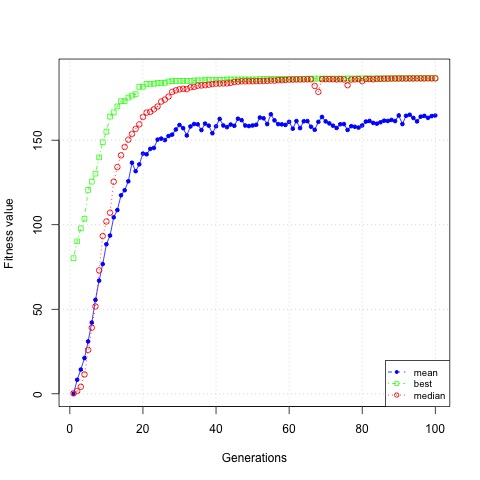
\includegraphics[width=3in]{{{inc/results/generations-Schubert-p050-i100-c0.25-m0.10-e0.05}}}\quad
}
\subfigure{
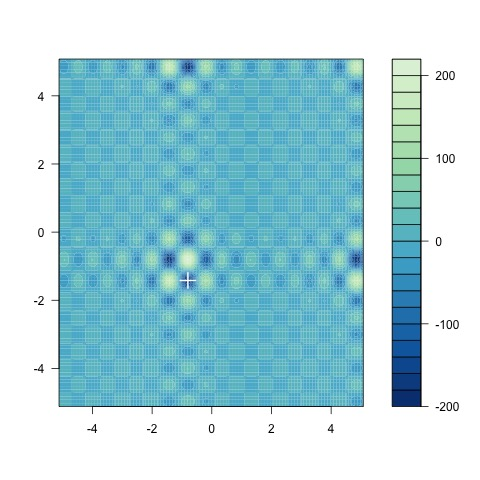
\includegraphics[width=3in]{{{inc/results/result-Schubert-p050-i100-c0.25-m0.10-e0.05}}}\quad
}
}
                 \caption{Test optymalizacji GA Schubert p50 i100 c0.25 m0.1 e0.05}
                 \end{figure}
\begin{figure}[!htbp]
    \centering
\mbox{
\subfigure{
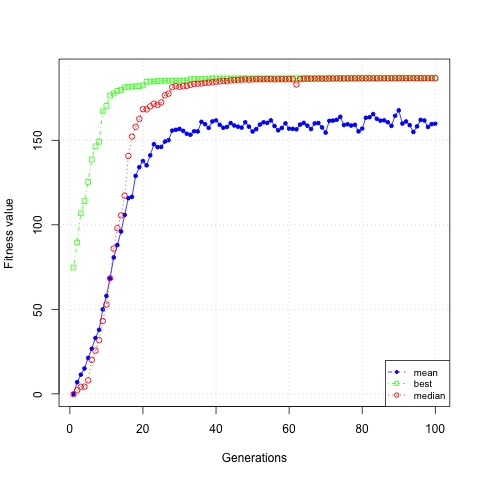
\includegraphics[width=3in]{{{inc/results/generations-Schubert-p050-i100-c0.50-m0.10-e0.05}}}\quad
}
\subfigure{
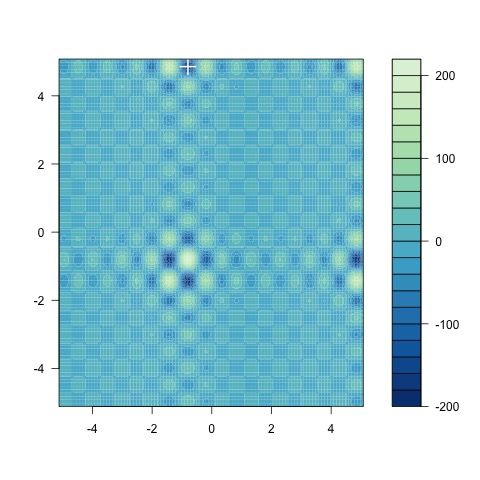
\includegraphics[width=3in]{{{inc/results/result-Schubert-p050-i100-c0.50-m0.10-e0.05}}}\quad
}
}
                 \caption{Test optymalizacji GA Schubert p50 i100 c0.5 m0.1 e0.05}
                 \end{figure}
\begin{figure}[!htbp]
    \centering
\mbox{
\subfigure{
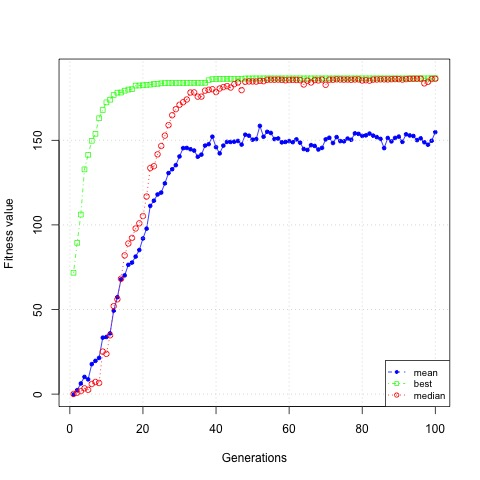
\includegraphics[width=3in]{{{inc/results/generations-Schubert-p050-i100-c0.75-m0.10-e0.05}}}\quad
}
\subfigure{
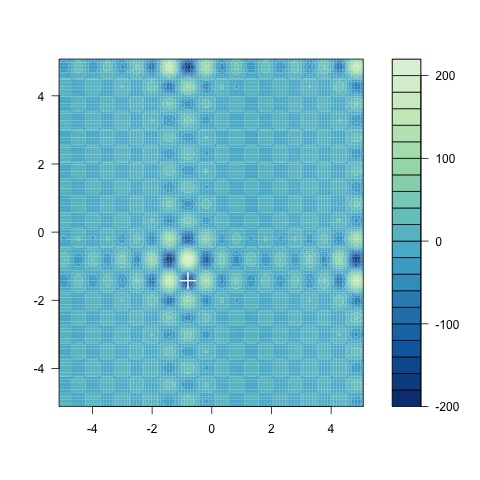
\includegraphics[width=3in]{{{inc/results/result-Schubert-p050-i100-c0.75-m0.10-e0.05}}}\quad
}
}
                 \caption{Test optymalizacji GA Schubert p50 i100 c0.75 m0.1 e0.05}
                 \end{figure}
\begin{figure}[!htbp]
    \centering
\mbox{
\subfigure{
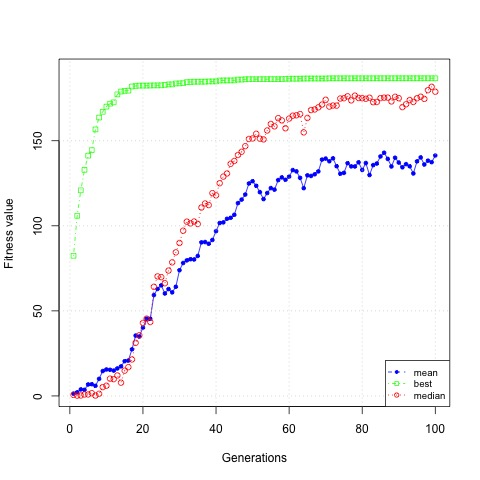
\includegraphics[width=3in]{{{inc/results/generations-Schubert-p050-i100-c1.00-m0.10-e0.05}}}\quad
}
\subfigure{
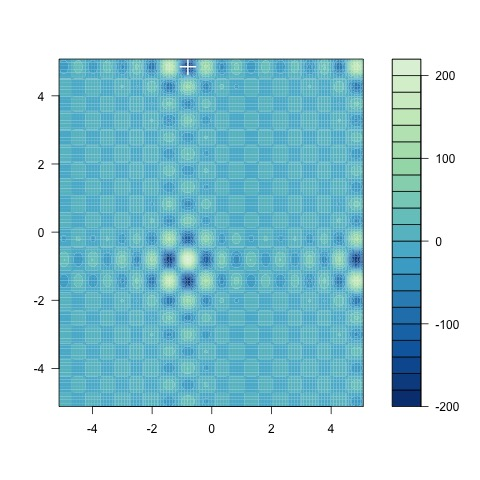
\includegraphics[width=3in]{{{inc/results/result-Schubert-p050-i100-c1.00-m0.10-e0.05}}}\quad
}
}
                 \caption{Test optymalizacji GA Schubert p50 i100 c1 m0.1 e0.05}
                 \end{figure}
   
  \clearpage
\subsubsection{Modyfikacja parametru liczby iteracji}        
W przypadku zwiększania ilości iteracji zarówno średnia jak i mediana pozostają na podobnym poziomie. Zmiana parametru liczby iteracji nie wpływa również znacząco na wyniki.                  
             
\begin{figure}[!htbp]
    \centering
\mbox{
\subfigure{
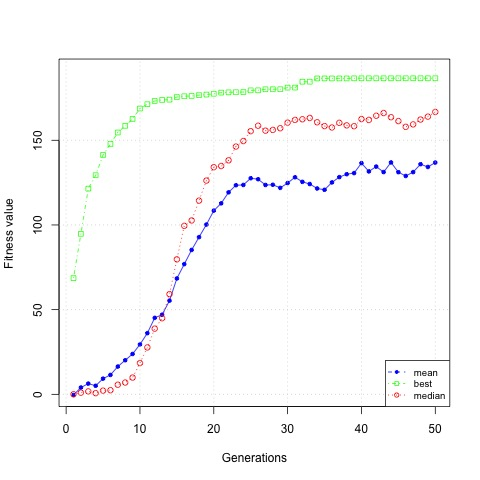
\includegraphics[width=3in]{{{inc/results/generations-Schubert-p050-i050-c0.80-m0.10-e0.05}}}\quad
}
\subfigure{
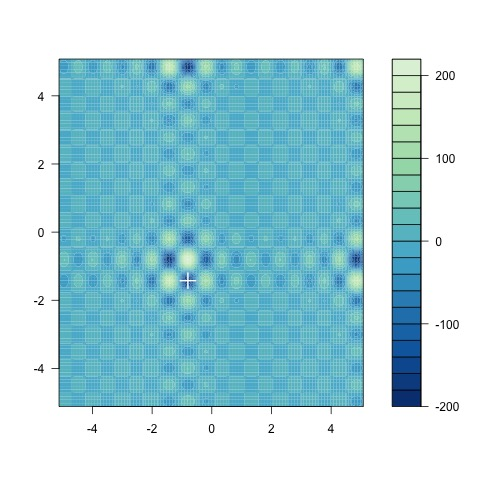
\includegraphics[width=3in]{{{inc/results/result-Schubert-p050-i050-c0.80-m0.10-e0.05}}}\quad
}
}
                 \caption{Test optymalizacji GA Schubert p50 i50 c0.8 m0.1 e0.05}
                 \end{figure}
\begin{figure}[!htbp]
    \centering
\mbox{
\subfigure{
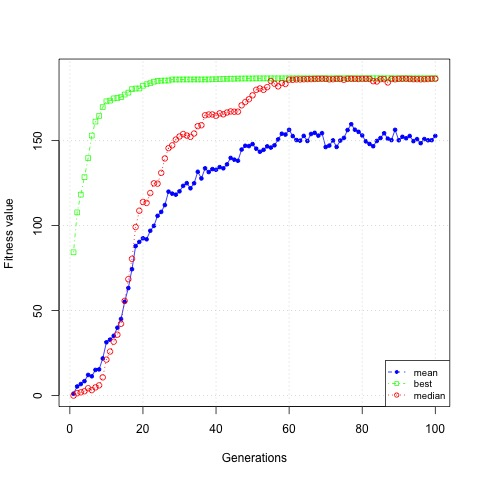
\includegraphics[width=3in]{{{inc/results/generations-Schubert-p050-i100-c0.80-m0.10-e0.05}}}\quad
}
\subfigure{
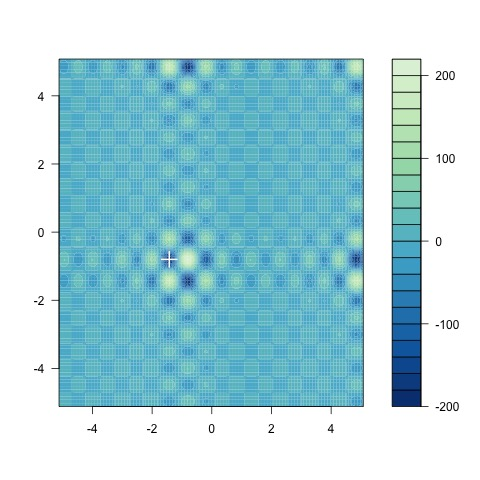
\includegraphics[width=3in]{{{inc/results/result-Schubert-p050-i100-c0.80-m0.10-e0.05}}}\quad
}
}
                 \caption{Test optymalizacji GA Schubert p50 i100 c0.8 m0.1 e0.05}
                 \end{figure}
\begin{figure}[!htbp]
    \centering
\mbox{
\subfigure{
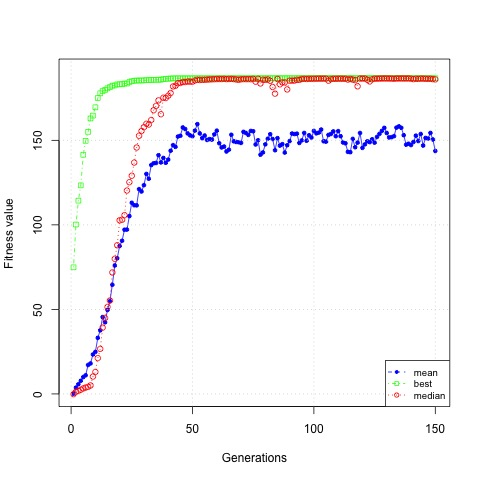
\includegraphics[width=3in]{{{inc/results/generations-Schubert-p050-i150-c0.80-m0.10-e0.05}}}\quad
}
\subfigure{
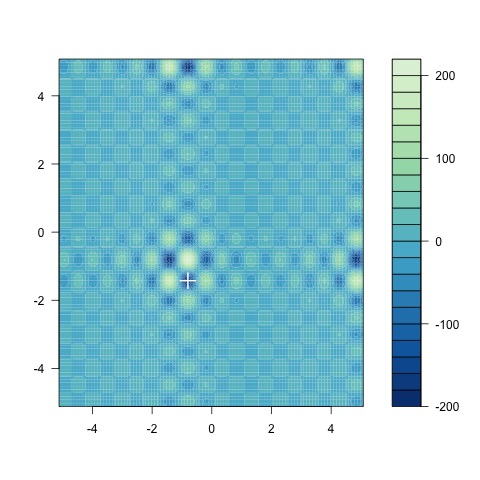
\includegraphics[width=3in]{{{inc/results/result-Schubert-p050-i150-c0.80-m0.10-e0.05}}}\quad
}
}
                 \caption{Test optymalizacji GA Schubert p50 i150 c0.8 m0.1 e0.05}
                 \end{figure}
\begin{figure}[!htbp]
    \centering
\mbox{
\subfigure{
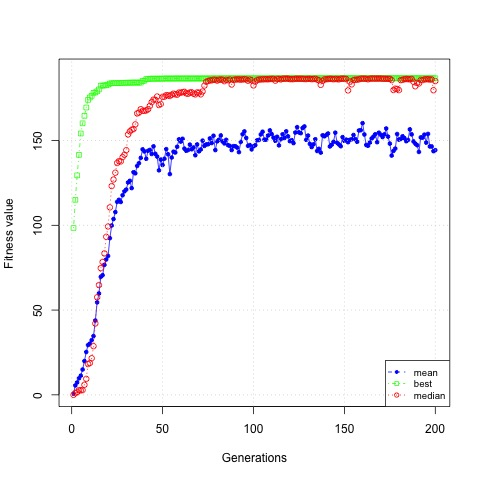
\includegraphics[width=3in]{{{inc/results/generations-Schubert-p050-i200-c0.80-m0.10-e0.05}}}\quad
}
\subfigure{
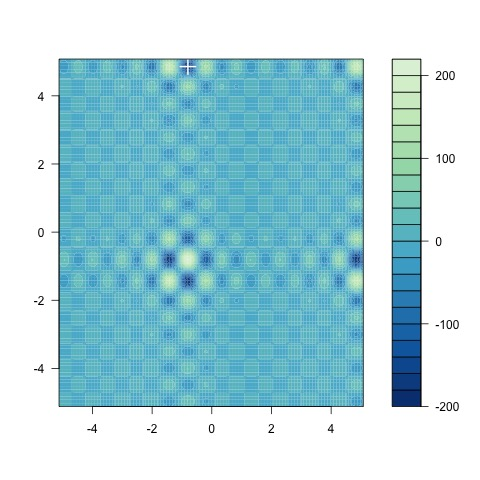
\includegraphics[width=3in]{{{inc/results/result-Schubert-p050-i200-c0.80-m0.10-e0.05}}}\quad
}
}
                 \caption{Test optymalizacji GA Schubert p50 i200 c0.8 m0.1 e0.05}
                 \end{figure}
\begin{figure}[!htbp]
    \centering
\mbox{
\subfigure{
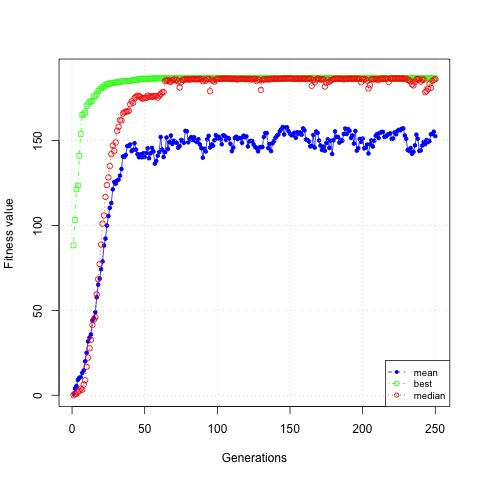
\includegraphics[width=3in]{{{inc/results/generations-Schubert-p050-i250-c0.80-m0.10-e0.05}}}\quad
}
\subfigure{
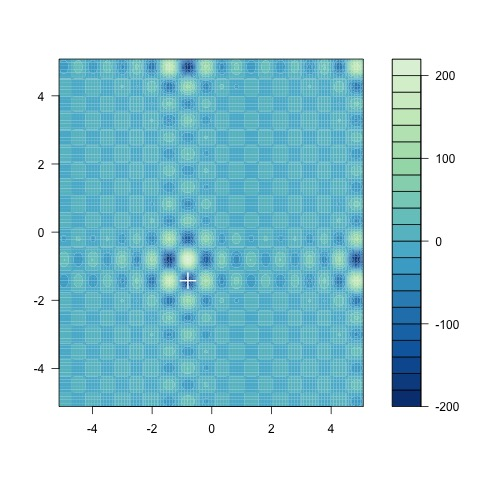
\includegraphics[width=3in]{{{inc/results/result-Schubert-p050-i250-c0.80-m0.10-e0.05}}}\quad
}
}
                 \caption{Test optymalizacji GA Schubert p50 i250 c0.8 m0.1 e0.05}
                 \end{figure}
                 
 \clearpage
\subsubsection{Modyfikacja parametru rozmiaru populacji}              

                 
Gdy parametr rozmiaru populacji jest ustawiony na wartość populacji 250 można zaobserwować mała anomalię średniej i mediany w okolicach 50-60 pokolenia. Anomalie średniej i mediany są skorelowane ze sobą, jednak nie wpływają na znalezione rozwiązanie. Niezależnie od rozmiaru parametru algorytm znajduje minimum globalne przy podobnej ilości pokoleń.                 
                 
                 
\begin{figure}[!htbp]
    \centering
\mbox{
\subfigure{
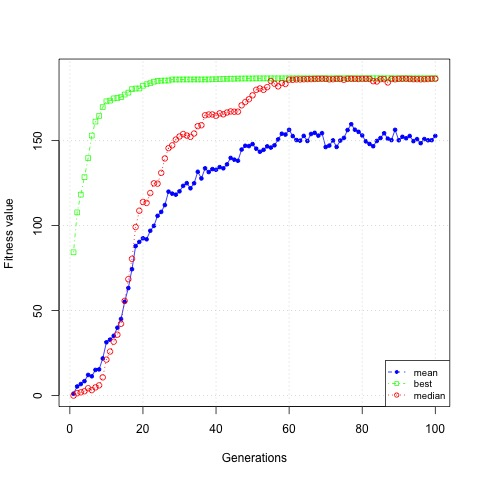
\includegraphics[width=3in]{{{inc/results/generations-Schubert-p050-i100-c0.80-m0.10-e0.05}}}\quad
}
\subfigure{
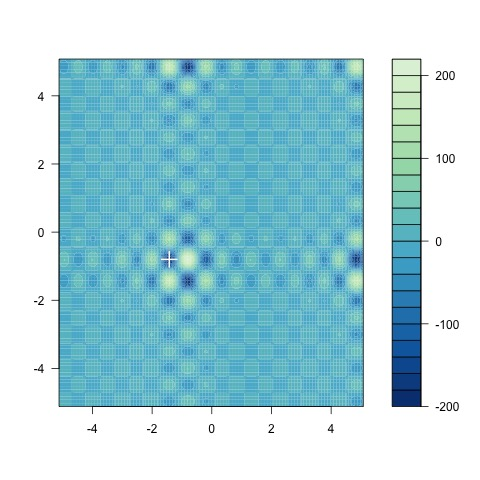
\includegraphics[width=3in]{{{inc/results/result-Schubert-p050-i100-c0.80-m0.10-e0.05}}}\quad
}
}
                 \caption{Test optymalizacji GA Schubert p50 i100 c0.8 m0.1 e0.05}
                 \end{figure}
\begin{figure}[!htbp]
    \centering
\mbox{
\subfigure{
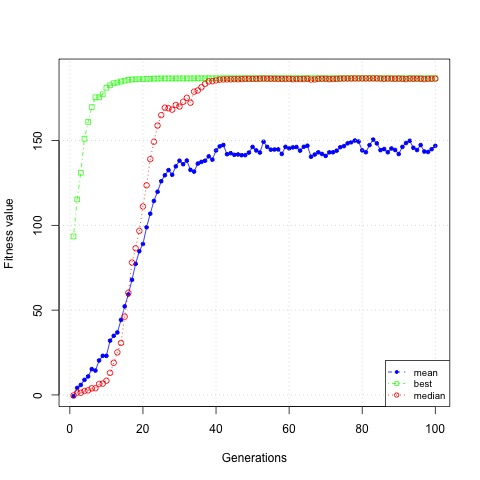
\includegraphics[width=3in]{{{inc/results/generations-Schubert-p100-i100-c0.80-m0.10-e0.05}}}\quad
}
\subfigure{
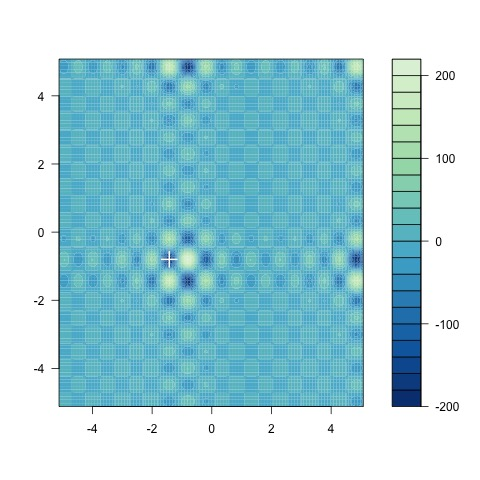
\includegraphics[width=3in]{{{inc/results/result-Schubert-p100-i100-c0.80-m0.10-e0.05}}}\quad
}
}
                 \caption{Test optymalizacji GA Schubert p100 i100 c0.8 m0.1 e0.05}
                 \end{figure}
\begin{figure}[!htbp]
    \centering
\mbox{
\subfigure{
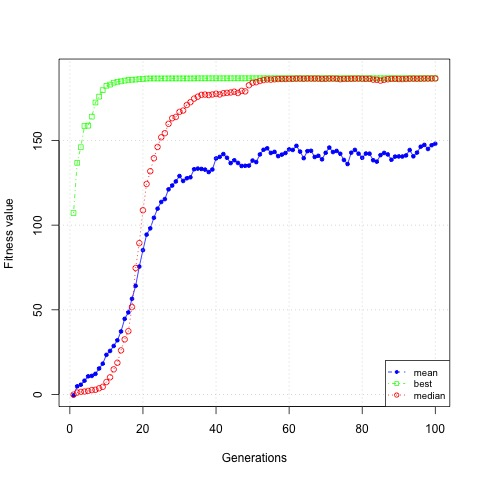
\includegraphics[width=3in]{{{inc/results/generations-Schubert-p150-i100-c0.80-m0.10-e0.05}}}\quad
}
\subfigure{
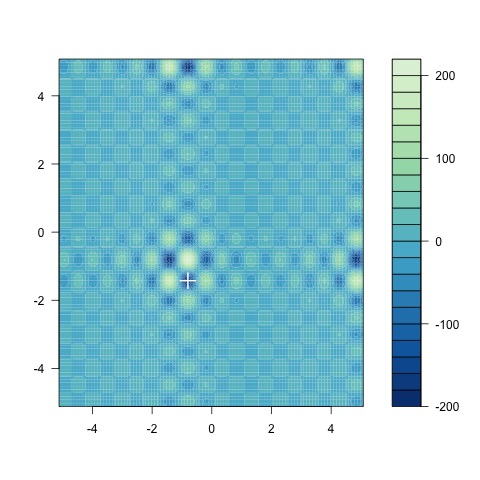
\includegraphics[width=3in]{{{inc/results/result-Schubert-p150-i100-c0.80-m0.10-e0.05}}}\quad
}
}
                 \caption{Test optymalizacji GA Schubert p150 i100 c0.8 m0.1 e0.05}
                 \end{figure}
\begin{figure}[!htbp]
    \centering
\mbox{
\subfigure{
\includegraphics[width=3in]{{{inc/results/generations-Schubert-p200-i100-c0.80-m0.10-e0.05}}}\quad
}
\subfigure{
\includegraphics[width=3in]{{{inc/results/result-Schubert-p200-i100-c0.80-m0.10-e0.05}}}\quad
}
}
                 \caption{Test optymalizacji GA Schubert p200 i100 c0.8 m0.1 e0.05}
                 \end{figure}

\begin{figure}[!htbp]
    \centering
\mbox{
\subfigure{
\includegraphics[width=3in]{{{inc/results/generations-Schubert-p250-i100-c0.80-m0.10-e0.05}}}\quad
}
\subfigure{
\includegraphics[width=3in]{{{inc/results/result-Schubert-p250-i100-c0.80-m0.10-e0.05}}}\quad
}
}
                 \caption{Test optymalizacji GA Schubert p250 i100 c0.8 m0.1 e0.05}
                 \end{figure}

                 
 \clearpage   
\subsection{Jednoczesna modyfikacja parametru krzyżowania i mutacji}     
     
 W przypadku jednoczesnej modyfikacji parametru krzyżowania i mutacji wyniki mają charakter losowy, lecz skupiają się wokół minimum lokalnych. Wraz ze wzrostem obydwu parametrów wartości średniej i mediany maleją.
 
 
 
\begin{figure}[!htbp]
    \centering
\mbox{
\subfigure{
\includegraphics[width=3in]{{{inc/results/generations-Schubert-p050-i100-c0.00-m0.00-e0.05}}}\quad
}
\subfigure{
\includegraphics[width=3in]{{{inc/results/result-Schubert-p050-i100-c0.00-m0.00-e0.05}}}\quad
}
}
                 \caption{Test optymalizacji GA Schubert p050 i100 c0.0 m0.0 e0.05}
\end{figure}


\begin{figure}[!htbp]
    \centering
\mbox{
\subfigure{
\includegraphics[width=3in]{{{inc/results/generations-Schubert-p050-i100-c0.25-m0.25-e0.05}}}\quad
}
\subfigure{
\includegraphics[width=3in]{{{inc/results/result-Schubert-p050-i100-c0.25-m0.25-e0.05}}}\quad
}
}
                 \caption{Test optymalizacji GA Schubert p050 i100 c0.25 m0.25 e0.05}
\end{figure}

               
               
\begin{figure}[!htbp]
    \centering
\mbox{
\subfigure{
\includegraphics[width=3in]{{{inc/results/generations-Schubert-p050-i100-c0.50-m0.50-e0.05}}}\quad
}
\subfigure{
\includegraphics[width=3in]{{{inc/results/result-Schubert-p050-i100-c0.50-m0.50-e0.05}}}\quad
}
}
                 \caption{Test optymalizacji GA Schubert p050 i100 c0.50 m0.50 e0.05}
\end{figure}


\begin{figure}[!htbp]
    \centering
\mbox{
\subfigure{
\includegraphics[width=3in]{{{inc/results/generations-Schubert-p050-i100-c0.75-m0.75-e0.05}}}\quad
}
\subfigure{
\includegraphics[width=3in]{{{inc/results/result-Schubert-p050-i100-c0.75-m0.75-e0.05}}}\quad
}
}
                 \caption{Test optymalizacji GA Schubert p050 i100 c0.75 m0.75 e0.05}
\end{figure}
     
 \begin{figure}[!htbp]
    \centering
\mbox{
\subfigure{
\includegraphics[width=3in]{{{inc/results/generations-Schubert-p050-i100-c1.00-m1.00-e0.05}}}\quad
}
\subfigure{
\includegraphics[width=3in]{{{inc/results/result-Schubert-p050-i100-c1.00-m1.00-e0.05}}}\quad
}
}
                 \caption{Test optymalizacji GA Schubert p050 i100 c1.00 m1.00 e0.05}
\end{figure}
    
     
                 
\clearpage
\section{Funkcja Bohachevsky'ego}
\subsection{Wzór analityczny}
\begin{figure}[!htbp]
    \centering
    \includegraphics[width=0.7\textwidth]{inc/wzory/bohachevsky}
     \caption{Wzór analityczny funkcji Bochachevsky'ego}
    \end{figure}
    
    \subsection{Wykres funkcji}
    \begin{figure}[!htbp]
    \centering
    \includegraphics[width=0.7\textwidth]{inc/wykresyfunkcji/bohachevsky}
     \caption{Wzór analityczny funkcji Bochachevsky'ego}
    \end{figure}
    
    \subsection{Ekstremum globalne}
    
     \begin{figure}[!htbp]
    \centering
    \includegraphics[width=0.7\textwidth]{inc/wzory/bohachevsky-global-minimum}
     \caption{Minimum globalne funkcji Bochachevsky'ego}
    \end{figure}
    
     \begin{figure}[!htbp]
    \centering
    \includegraphics[width=0.7\textwidth]{inc/wykresyfunkcji/bohachevsky-global-minimum}
     \caption{Minimum globalne funkcji Bochachevsky'ego}
    \end{figure}
    
    
    \subsection{Optymalizacja}
\subsubsection{Modyfikacja parametru elitarności}    
W przypadku zwiększania wartości elitarności populacji średnia i mediana pozostają na podobnym poziomie. W przypadku większej elitarności algorytm szybciej znajduje optymalne rozwiązanie. Jeżeli elitarność populacji jest równa 1, to algorytm stochastycznie wylosował jeden zestaw rozwiązań, który z powodu braku ewolucji nie zbliżył się do rozwiązania optymalnego.

\begin{figure}[!htbp]
    \centering
\mbox{
\subfigure{
\includegraphics[width=3in]{{{inc/results/generations-Bohachevsky1-p050-i100-c0.80-m0.10-e0.00}}}\quad
}
\subfigure{
\includegraphics[width=3in]{{{inc/results/result-Bohachevsky1-p050-i100-c0.80-m0.10-e0.00}}}\quad
}
}
                 \caption{Test optymalizacji GA Bohachevsky1 p50 i100 c0.8 m0.1 e0}
                 \end{figure}
\begin{figure}[!htbp]
    \centering
\mbox{
\subfigure{
\includegraphics[width=3in]{{{inc/results/generations-Bohachevsky1-p050-i100-c0.80-m0.10-e0.25}}}\quad
}
\subfigure{
\includegraphics[width=3in]{{{inc/results/result-Bohachevsky1-p050-i100-c0.80-m0.10-e0.25}}}\quad
}
}
                 \caption{Test optymalizacji GA Bohachevsky1 p50 i100 c0.8 m0.1 e0.25}
                 \end{figure}
\begin{figure}[!htbp]
    \centering
\mbox{
\subfigure{
\includegraphics[width=3in]{{{inc/results/generations-Bohachevsky1-p050-i100-c0.80-m0.10-e0.50}}}\quad
}
\subfigure{
\includegraphics[width=3in]{{{inc/results/result-Bohachevsky1-p050-i100-c0.80-m0.10-e0.50}}}\quad
}
}
                 \caption{Test optymalizacji GA Bohachevsky1 p50 i100 c0.8 m0.1 e0.5}
                 \end{figure}
\begin{figure}[!htbp]
    \centering
\mbox{
\subfigure{
\includegraphics[width=3in]{{{inc/results/generations-Bohachevsky1-p050-i100-c0.80-m0.10-e0.75}}}\quad
}
\subfigure{
\includegraphics[width=3in]{{{inc/results/result-Bohachevsky1-p050-i100-c0.80-m0.10-e0.75}}}\quad
}
}
                 \caption{Test optymalizacji GA Bohachevsky1 p50 i100 c0.8 m0.1 e0.75}
                 \end{figure}
\begin{figure}[!htbp]
    \centering
\mbox{
\subfigure{
\includegraphics[width=3in]{{{inc/results/generations-Bohachevsky1-p050-i100-c0.80-m0.10-e1.00}}}\quad
}
\subfigure{
\includegraphics[width=3in]{{{inc/results/result-Bohachevsky1-p050-i100-c0.80-m0.10-e1.00}}}\quad
}
}
                 \caption{Test optymalizacji GA Bohachevsky1 p50 i100 c0.8 m0.1 e1}
                 \end{figure}


\clearpage
\subsubsection{Modyfikacja parametru mutacji}

 Zwiększanie parametru mutacji sprawia, że zarówno średnia jak i mediana zwiększają się wraz ze wzrostem parametru mutacji. Niezależnie od tego algorytm znajduje optymalne rozwiązanie stosunkowo szybko i po podobnej ilości pokoleń.
 
 
 
\begin{figure}[!htbp]
    \centering
\mbox{
\subfigure{
\includegraphics[width=3in]{{{inc/results/generations-Bohachevsky1-p050-i100-c0.80-m0.00-e0.05}}}\quad
}
\subfigure{
\includegraphics[width=3in]{{{inc/results/result-Bohachevsky1-p050-i100-c0.80-m0.00-e0.05}}}\quad
}
}
                 \caption{Test optymalizacji GA Bohachevsky1 p50 i100 c0.8 m0 e0.05}
                 \end{figure}
\begin{figure}[!htbp]
    \centering
\mbox{
\subfigure{
\includegraphics[width=3in]{{{inc/results/generations-Bohachevsky1-p050-i100-c0.80-m0.25-e0.05}}}\quad
}
\subfigure{
\includegraphics[width=3in]{{{inc/results/result-Bohachevsky1-p050-i100-c0.80-m0.25-e0.05}}}\quad
}
}
                 \caption{Test optymalizacji GA Bohachevsky1 p50 i100 c0.8 m0.25 e0.05}
                 \end{figure}
\begin{figure}[!htbp]
    \centering
\mbox{
\subfigure{
\includegraphics[width=3in]{{{inc/results/generations-Bohachevsky1-p050-i100-c0.80-m0.50-e0.05}}}\quad
}
\subfigure{
\includegraphics[width=3in]{{{inc/results/result-Bohachevsky1-p050-i100-c0.80-m0.50-e0.05}}}\quad
}
}
                 \caption{Test optymalizacji GA Bohachevsky1 p50 i100 c0.8 m0.5 e0.05}
                 \end{figure}
\begin{figure}[!htbp]
    \centering
\mbox{
\subfigure{
\includegraphics[width=3in]{{{inc/results/generations-Bohachevsky1-p050-i100-c0.80-m0.75-e0.05}}}\quad
}
\subfigure{
\includegraphics[width=3in]{{{inc/results/result-Bohachevsky1-p050-i100-c0.80-m0.75-e0.05}}}\quad
}
}
                 \caption{Test optymalizacji GA Bohachevsky1 p50 i100 c0.8 m0.75 e0.05}
                 \end{figure}
\begin{figure}[!htbp]
    \centering
\mbox{
\subfigure{
\includegraphics[width=3in]{{{inc/results/generations-Bohachevsky1-p050-i100-c0.80-m1.00-e0.05}}}\quad
}
\subfigure{
\includegraphics[width=3in]{{{inc/results/result-Bohachevsky1-p050-i100-c0.80-m1.00-e0.05}}}\quad
}
}
                 \caption{Test optymalizacji GA Bohachevsky1 p50 i100 c0.8 m1 e0.05}
                 \end{figure}
                 

\clearpage
\subsubsection{Modyfikacja parametru krzyżowania}

 Modyfikacja parametru krzyżowania nie wpływa na rozwiązanie, ani na wartości średniej i mediany. W odróżnieniu od funkcji Schuberta, funkcja Bohachevsky'ego  nie posiada wielu minimum lokalnych, a tylko jedno ekstremum, które okazuje się globalne.
                
\begin{figure}[!htbp]
    \centering
\mbox{
\subfigure{
\includegraphics[width=3in]{{{inc/results/generations-Bohachevsky1-p050-i100-c0.00-m0.10-e0.05}}}\quad
}
\subfigure{
\includegraphics[width=3in]{{{inc/results/result-Bohachevsky1-p050-i100-c0.00-m0.10-e0.05}}}\quad
}
}
                 \caption{Test optymalizacji GA Bohachevsky1 p50 i100 c0 m0.1 e0.05}
                 \end{figure}
\begin{figure}[!htbp]
    \centering
\mbox{
\subfigure{
\includegraphics[width=3in]{{{inc/results/generations-Bohachevsky1-p050-i100-c0.25-m0.10-e0.05}}}\quad
}
\subfigure{
\includegraphics[width=3in]{{{inc/results/result-Bohachevsky1-p050-i100-c0.25-m0.10-e0.05}}}\quad
}
}
                 \caption{Test optymalizacji GA Bohachevsky1 p50 i100 c0.25 m0.1 e0.05}
                 \end{figure}
\begin{figure}[!htbp]
    \centering
\mbox{
\subfigure{
\includegraphics[width=3in]{{{inc/results/generations-Bohachevsky1-p050-i100-c0.50-m0.10-e0.05}}}\quad
}
\subfigure{
\includegraphics[width=3in]{{{inc/results/result-Bohachevsky1-p050-i100-c0.50-m0.10-e0.05}}}\quad
}
}
                 \caption{Test optymalizacji GA Bohachevsky1 p50 i100 c0.5 m0.1 e0.05}
                 \end{figure}
\begin{figure}[!htbp]
    \centering
\mbox{
\subfigure{
\includegraphics[width=3in]{{{inc/results/generations-Bohachevsky1-p050-i100-c0.75-m0.10-e0.05}}}\quad
}
\subfigure{
\includegraphics[width=3in]{{{inc/results/result-Bohachevsky1-p050-i100-c0.75-m0.10-e0.05}}}\quad
}
}
                 \caption{Test optymalizacji GA Bohachevsky1 p50 i100 c0.75 m0.1 e0.05}
                 \end{figure}
\begin{figure}[!htbp]
    \centering
\mbox{
\subfigure{
\includegraphics[width=3in]{{{inc/results/generations-Bohachevsky1-p050-i100-c1.00-m0.10-e0.05}}}\quad
}
\subfigure{
\includegraphics[width=3in]{{{inc/results/result-Bohachevsky1-p050-i100-c1.00-m0.10-e0.05}}}\quad
}
}
                 \caption{Test optymalizacji GA Bohachevsky1 p50 i100 c1 m0.1 e0.05}
                 \end{figure}
 
        
 \clearpage
\subsubsection{Modyfikacja parametru liczby iteracji}              

Modyfikacja parametru liczby iteracji nie wpływa na rozwiązanie, ani na wartości średniej i mediany.                  
Sytuacja jest analogiczna do przypadku modyfikacji parametru krzyżowania.

\begin{figure}[!htbp]
    \centering
\mbox{
\subfigure{
\includegraphics[width=3in]{{{inc/results/generations-Bohachevsky1-p050-i050-c0.80-m0.10-e0.05}}}\quad
}
\subfigure{
\includegraphics[width=3in]{{{inc/results/result-Bohachevsky1-p050-i050-c0.80-m0.10-e0.05}}}\quad
}
}
                 \caption{Test optymalizacji GA Bohachevsky1 p50 i50 c0.8 m0.1 e0.05}
                 \end{figure}
\begin{figure}[!htbp]
    \centering
\mbox{
\subfigure{
\includegraphics[width=3in]{{{inc/results/generations-Bohachevsky1-p050-i100-c0.80-m0.10-e0.05}}}\quad
}
\subfigure{
\includegraphics[width=3in]{{{inc/results/result-Bohachevsky1-p050-i100-c0.80-m0.10-e0.05}}}\quad
}
}
                 \caption{Test optymalizacji GA Bohachevsky1 p50 i100 c0.8 m0.1 e0.05}
                 \end{figure}
\begin{figure}[!htbp]
    \centering
\mbox{
\subfigure{
\includegraphics[width=3in]{{{inc/results/generations-Bohachevsky1-p050-i150-c0.80-m0.10-e0.05}}}\quad
}
\subfigure{
\includegraphics[width=3in]{{{inc/results/result-Bohachevsky1-p050-i150-c0.80-m0.10-e0.05}}}\quad
}
}
                 \caption{Test optymalizacji GA Bohachevsky1 p50 i150 c0.8 m0.1 e0.05}
                 \end{figure}
\begin{figure}[!htbp]
    \centering
\mbox{
\subfigure{
\includegraphics[width=3in]{{{inc/results/generations-Bohachevsky1-p050-i200-c0.80-m0.10-e0.05}}}\quad
}
\subfigure{
\includegraphics[width=3in]{{{inc/results/result-Bohachevsky1-p050-i200-c0.80-m0.10-e0.05}}}\quad
}
}
                 \caption{Test optymalizacji GA Bohachevsky1 p50 i200 c0.8 m0.1 e0.05}
                 \end{figure}
\begin{figure}[!htbp]
    \centering
\mbox{
\subfigure{
\includegraphics[width=3in]{{{inc/results/generations-Bohachevsky1-p050-i250-c0.80-m0.10-e0.05}}}\quad
}
\subfigure{
\includegraphics[width=3in]{{{inc/results/result-Bohachevsky1-p050-i250-c0.80-m0.10-e0.05}}}\quad
}
}
                 \caption{Test optymalizacji GA Bohachevsky1 p50 i250 c0.8 m0.1 e0.05}
                 \end{figure}
 \clearpage            
  
\subsubsection{Modyfikacja parametru rozmiaru populacji}              
 Modyfikacja parametru rozmiaru populacji  nie wpływa na rozwiązanie, ani na wartości średniej i mediany. Sytuacja jest analogiczna do przypadku modyfikacji parametru krzyżowania.   
\begin{figure}[!htbp]
    \centering
\mbox{
\subfigure{
\includegraphics[width=3in]{{{inc/results/generations-Bohachevsky1-p050-i100-c0.80-m0.10-e0.05}}}\quad
}
\subfigure{
\includegraphics[width=3in]{{{inc/results/result-Bohachevsky1-p050-i100-c0.80-m0.10-e0.05}}}\quad
}
}
                 \caption{Test optymalizacji GA Bohachevsky1 p50 i100 c0.8 m0.1 e0.05}
                 \end{figure}
                 
                              
\begin{figure}[!htbp]
    \centering
\mbox{
\subfigure{
\includegraphics[width=3in]{{{inc/results/generations-Bohachevsky1-p100-i100-c0.80-m0.10-e0.05}}}\quad
}
\subfigure{
\includegraphics[width=3in]{{{inc/results/result-Bohachevsky1-p100-i100-c0.80-m0.10-e0.05}}}\quad
}
}
                 \caption{Test optymalizacji GA Bohachevsky1 p100 i100 c0.8 m0.1 e0.05}
                 \end{figure}
\begin{figure}[!htbp]
    \centering
\mbox{
\subfigure{
\includegraphics[width=3in]{{{inc/results/generations-Bohachevsky1-p150-i100-c0.80-m0.10-e0.05}}}\quad
}
\subfigure{
\includegraphics[width=3in]{{{inc/results/result-Bohachevsky1-p150-i100-c0.80-m0.10-e0.05}}}\quad
}
}
                 \caption{Test optymalizacji GA Bohachevsky1 p150 i100 c0.8 m0.1 e0.05}
                 \end{figure}
\begin{figure}[!htbp]
    \centering
\mbox{
\subfigure{
\includegraphics[width=3in]{{{inc/results/generations-Bohachevsky1-p200-i100-c0.80-m0.10-e0.05}}}\quad
}
\subfigure{
\includegraphics[width=3in]{{{inc/results/result-Bohachevsky1-p200-i100-c0.80-m0.10-e0.05}}}\quad
}
}
                 \caption{Test optymalizacji GA Bohachevsky1 p200 i100 c0.8 m0.1 e0.05}
                 \end{figure}
\begin{figure}[!htbp]
    \centering
\mbox{
\subfigure{
\includegraphics[width=3in]{{{inc/results/generations-Bohachevsky1-p250-i100-c0.80-m0.10-e0.05}}}\quad
}
\subfigure{
\includegraphics[width=3in]{{{inc/results/result-Bohachevsky1-p250-i100-c0.80-m0.10-e0.05}}}\quad
}
}
                 \caption{Test optymalizacji GA Bohachevsky1 p250 i100 c0.8 m0.1 e0.05}
                 \end{figure}
                 
  \clearpage   
\subsection{Jednoczesna modyfikacja parametru krzyżowania i mutacji}     
     
     W przypadku jednoczesnej modyfikacji parametru krzyżowania i mutacji krzywe rozwiązania mają wartości podobne. Wraz ze wzrostem obydwu parametrów wartości średniej i mediany są gorsze. 
 
 
 
\begin{figure}[!htbp]
    \centering
\mbox{
\subfigure{
\includegraphics[width=3in]{{{inc/results/generations-Bohachevsky1-p050-i100-c0.00-m0.00-e0.05}}}\quad
}
\subfigure{
\includegraphics[width=3in]{{{inc/results/result-Bohachevsky1-p050-i100-c0.00-m0.00-e0.05}}}\quad
}
}
                 \caption{Test optymalizacji GA Bohachevsky1 p050 i100 c0.0 m0.0 e0.05}
\end{figure}


\begin{figure}[!htbp]
    \centering
\mbox{
\subfigure{
\includegraphics[width=3in]{{{inc/results/generations-Bohachevsky1-p050-i100-c0.25-m0.25-e0.05}}}\quad
}
\subfigure{
\includegraphics[width=3in]{{{inc/results/result-Bohachevsky1-p050-i100-c0.25-m0.25-e0.05}}}\quad
}
}
                 \caption{Test optymalizacji GA Bohachevsky1 p050 i100 c0.25 m0.25 e0.05}
\end{figure}

               
               
\begin{figure}[!htbp]
    \centering
\mbox{
\subfigure{
\includegraphics[width=3in]{{{inc/results/generations-Bohachevsky1-p050-i100-c0.50-m0.50-e0.05}}}\quad
}
\subfigure{
\includegraphics[width=3in]{{{inc/results/result-Bohachevsky1-p050-i100-c0.50-m0.50-e0.05}}}\quad
}
}
                 \caption{Test optymalizacji GA Bohachevsky1 p050 i100 c0.50 m0.50 e0.05}
\end{figure}


\begin{figure}[!htbp]
    \centering
\mbox{
\subfigure{
\includegraphics[width=3in]{{{inc/results/generations-Bohachevsky1-p050-i100-c0.75-m0.75-e0.05}}}\quad
}
\subfigure{
\includegraphics[width=3in]{{{inc/results/result-Bohachevsky1-p050-i100-c0.75-m0.75-e0.05}}}\quad
}
}
                 \caption{Test optymalizacji GA Bohachevsky1 p050 i100 c0.75 m0.75 e0.05}
\end{figure}
     
 \begin{figure}[!htbp]
    \centering
\mbox{
\subfigure{
\includegraphics[width=3in]{{{inc/results/generations-Bohachevsky1-p050-i100-c1.00-m1.00-e0.05}}}\quad
}
\subfigure{
\includegraphics[width=3in]{{{inc/results/result-Bohachevsky1-p050-i100-c1.00-m1.00-e0.05}}}\quad
}
}
                 \caption{Test optymalizacji GA Bohachevsky1 p050 i100 c1.00 m1.00 e0.05}
\end{figure}         
          
          
          
                 
 \clearpage                
\newpage
\section{Funkcja Branina}
\subsection{Wzór analityczny}
\begin{figure}[!htbp]
    \centering
    \includegraphics[width=0.7\textwidth]{inc/wzory/branin}
     \caption{Wzór analityczny funkcji Branina}
    \end{figure}                 

    
\subsection{Wykres w ustalonym przedziale zmiennych  }
       \begin{figure}[!htbp]
    \centering
    \includegraphics[width=0.7\textwidth]{inc/wykresyfunkcji/branin}
     \caption{Wzór analityczny funkcji Branina}
    \end{figure}                 

\subsection{Ekstremum globalne}
\begin{figure}[!htbp]
    \centering
    \includegraphics[width=0.7\textwidth]{inc/wzory/branin-global-minimum}
     \caption{Minimum globalne funkcji Branina}
    \end{figure}             
    
 
 \begin{figure}[!htbp]
    \centering
    \includegraphics[width=0.7\textwidth]{inc/wykresyfunkcji/branin-global-minimum}
     \caption{Minimum globalne funkcji Branina}
    \end{figure}             
    
       
\subsection{Optymalizacja}            

\subsubsection{Modyfikacja parametru elitarności}    

W przypadku braku populacji elitarnej algorytm potrzebował więcej czasu aby odnaleźć poprawny wynik, wskazuje na to wykres mediany. W przypadku wartości 0.25, 0.5 oraz 0.75 algorytm szybciej odnajdywał poprawne rozwiązanie. W momencie gdy cała populacje była oznaczana jako elitarna algorytm nie znajdował poprawnego rozwiązania, nie występowała również zmiana między kolejnymi generacjami. 

\begin{figure}[!htbp]
    \centering
\mbox{
\subfigure{
\includegraphics[width=3in]{{{inc/results/generations-Branin-p050-i100-c0.80-m0.10-e0.00}}}\quad
}
\subfigure{
\includegraphics[width=3in]{{{inc/results/result-Branin-p050-i100-c0.80-m0.10-e0.00}}}\quad
}
}
                 \caption{Test optymalizacji GA Branin p50 i100 c0.8 m0.1 e0}
                 \end{figure}
\begin{figure}[!htbp]
    \centering
\mbox{
\subfigure{
\includegraphics[width=3in]{{{inc/results/generations-Branin-p050-i100-c0.80-m0.10-e0.25}}}\quad
}
\subfigure{
\includegraphics[width=3in]{{{inc/results/result-Branin-p050-i100-c0.80-m0.10-e0.25}}}\quad
}
}
                 \caption{Test optymalizacji GA Branin p50 i100 c0.8 m0.1 e0.25}
                 \end{figure}
\begin{figure}[!htbp]
    \centering
\mbox{
\subfigure{
\includegraphics[width=3in]{{{inc/results/generations-Branin-p050-i100-c0.80-m0.10-e0.50}}}\quad
}
\subfigure{
\includegraphics[width=3in]{{{inc/results/result-Branin-p050-i100-c0.80-m0.10-e0.50}}}\quad
}
}
                 \caption{Test optymalizacji GA Branin p50 i100 c0.8 m0.1 e0.5}
                 \end{figure}
\begin{figure}[!htbp]
    \centering
\mbox{
\subfigure{
\includegraphics[width=3in]{{{inc/results/generations-Branin-p050-i100-c0.80-m0.10-e0.75}}}\quad
}
\subfigure{
\includegraphics[width=3in]{{{inc/results/result-Branin-p050-i100-c0.80-m0.10-e0.75}}}\quad
}
}
                 \caption{Test optymalizacji GA Branin p50 i100 c0.8 m0.1 e0.75}
                 \end{figure}
\begin{figure}[!htbp]
    \centering
\mbox{
\subfigure{
\includegraphics[width=3in]{{{inc/results/generations-Branin-p050-i100-c0.80-m0.10-e1.00}}}\quad
}
\subfigure{
\includegraphics[width=3in]{{{inc/results/result-Branin-p050-i100-c0.80-m0.10-e1.00}}}\quad
}
}
                 \caption{Test optymalizacji GA Branin p50 i100 c0.8 m0.1 e1}
                 \end{figure}
               
  \clearpage
 \subsubsection{Modyfikacja parametru mutacji}
 Algorytm bez względu na zmianę parametru mutacji zawsze odnajdował poprawne rozwiązanie, im większa wartość parametru tym wykres mediany oraz średniej wskazywał na coraz większe odchylenia i niższe wyniki.

\begin{figure}[!htbp]
    \centering
\mbox{
\subfigure{
\includegraphics[width=3in]{{{inc/results/generations-Branin-p050-i100-c0.80-m0.00-e0.05}}}\quad
}
\subfigure{
\includegraphics[width=3in]{{{inc/results/result-Branin-p050-i100-c0.80-m0.00-e0.05}}}\quad
}
}
                 \caption{Test optymalizacji GA Branin p50 i100 c0.8 m0 e0.05}
                 \end{figure}
\begin{figure}[!htbp]
    \centering
\mbox{
\subfigure{
\includegraphics[width=3in]{{{inc/results/generations-Branin-p050-i100-c0.80-m0.25-e0.05}}}\quad
}
\subfigure{
\includegraphics[width=3in]{{{inc/results/result-Branin-p050-i100-c0.80-m0.25-e0.05}}}\quad
}
}
                 \caption{Test optymalizacji GA Branin p50 i100 c0.8 m0.25 e0.05}
                 \end{figure}
\begin{figure}[!htbp]
    \centering
\mbox{
\subfigure{
\includegraphics[width=3in]{{{inc/results/generations-Branin-p050-i100-c0.80-m0.50-e0.05}}}\quad
}
\subfigure{
\includegraphics[width=3in]{{{inc/results/result-Branin-p050-i100-c0.80-m0.50-e0.05}}}\quad
}
}
                 \caption{Test optymalizacji GA Branin p50 i100 c0.8 m0.5 e0.05}
                 \end{figure}
\begin{figure}[!htbp]
    \centering
\mbox{
\subfigure{
\includegraphics[width=3in]{{{inc/results/generations-Branin-p050-i100-c0.80-m0.75-e0.05}}}\quad
}
\subfigure{
\includegraphics[width=3in]{{{inc/results/result-Branin-p050-i100-c0.80-m0.75-e0.05}}}\quad
}
}
                 \caption{Test optymalizacji GA Branin p50 i100 c0.8 m0.75 e0.05}
                 \end{figure}
\begin{figure}[!htbp]
    \centering
\mbox{
\subfigure{
\includegraphics[width=3in]{{{inc/results/generations-Branin-p050-i100-c0.80-m1.00-e0.05}}}\quad
}
\subfigure{
\includegraphics[width=3in]{{{inc/results/result-Branin-p050-i100-c0.80-m1.00-e0.05}}}\quad
}
}
                 \caption{Test optymalizacji GA Branin p50 i100 c0.8 m1 e0.05}
                 \end{figure}
                 
 \clearpage
\subsubsection{Modyfikacja parametru krzyżowania}             
W przypadku braku krzyżowania funkcja potrzebuje większej ilości iteracji aby znaleźć poprawne rozwiązanie. Wyższy wskaźnik ma w tym przypadku pozytywny wpływ na szybkość odnajdywanego rozwiązania.
\begin{figure}[!htbp]
    \centering
\mbox{
\subfigure{
\includegraphics[width=3in]{{{inc/results/generations-Branin-p050-i100-c0.00-m0.10-e0.05}}}\quad
}
\subfigure{
\includegraphics[width=3in]{{{inc/results/result-Branin-p050-i100-c0.00-m0.10-e0.05}}}\quad
}
}
                 \caption{Test optymalizacji GA Branin p50 i100 c0 m0.1 e0.05}
                 \end{figure}
\begin{figure}[!htbp]
    \centering
\mbox{
\subfigure{
\includegraphics[width=3in]{{{inc/results/generations-Branin-p050-i100-c0.25-m0.10-e0.05}}}\quad
}
\subfigure{
\includegraphics[width=3in]{{{inc/results/result-Branin-p050-i100-c0.25-m0.10-e0.05}}}\quad
}
}
                 \caption{Test optymalizacji GA Branin p50 i100 c0.25 m0.1 e0.05}
                 \end{figure}
\begin{figure}[!htbp]
    \centering
\mbox{
\subfigure{
\includegraphics[width=3in]{{{inc/results/generations-Branin-p050-i100-c0.50-m0.10-e0.05}}}\quad
}
\subfigure{
\includegraphics[width=3in]{{{inc/results/result-Branin-p050-i100-c0.50-m0.10-e0.05}}}\quad
}
}
                 \caption{Test optymalizacji GA Branin p50 i100 c0.5 m0.1 e0.05}
                 \end{figure}
\begin{figure}[!htbp]
    \centering
\mbox{
\subfigure{
\includegraphics[width=3in]{{{inc/results/generations-Branin-p050-i100-c0.75-m0.10-e0.05}}}\quad
}
\subfigure{
\includegraphics[width=3in]{{{inc/results/result-Branin-p050-i100-c0.75-m0.10-e0.05}}}\quad
}
}
                 \caption{Test optymalizacji GA Branin p50 i100 c0.75 m0.1 e0.05}
                 \end{figure}
\begin{figure}[!htbp]
    \centering
\mbox{
\subfigure{
\includegraphics[width=3in]{{{inc/results/generations-Branin-p050-i100-c1.00-m0.10-e0.05}}}\quad
}
\subfigure{
\includegraphics[width=3in]{{{inc/results/result-Branin-p050-i100-c1.00-m0.10-e0.05}}}\quad
}
}
                 \caption{Test optymalizacji GA Branin p50 i100 c1 m0.1 e0.05}
                 \end{figure}
                 
                 
\clearpage
\subsubsection{Modyfikacja parametru liczby iteracji}              
Zmiana liczby iteracji w przypadku funkcji Branin nie wpływa na jakość rozwiązania. Nie występują żadne anomalie między zmianami parametru. Funkcja w każdym przypadku zachowuję się identycznie. 
\begin{figure}[!htbp]
    \centering
\mbox{
\subfigure{
\includegraphics[width=3in]{{{inc/results/generations-Branin-p050-i050-c0.80-m0.10-e0.05}}}\quad
}
\subfigure{
\includegraphics[width=3in]{{{inc/results/result-Branin-p050-i050-c0.80-m0.10-e0.05}}}\quad
}
}
                 \caption{Test optymalizacji GA Branin p50 i50 c0.8 m0.1 e0.05}
                 \end{figure}
\begin{figure}[!htbp]
    \centering
\mbox{
\subfigure{
\includegraphics[width=3in]{{{inc/results/generations-Branin-p050-i100-c0.80-m0.10-e0.05}}}\quad
}
\subfigure{
\includegraphics[width=3in]{{{inc/results/result-Branin-p050-i100-c0.80-m0.10-e0.05}}}\quad
}
}
                 \caption{Test optymalizacji GA Branin p50 i100 c0.8 m0.1 e0.05}
                 \end{figure}
\begin{figure}[!htbp]
    \centering
\mbox{
\subfigure{
\includegraphics[width=3in]{{{inc/results/generations-Branin-p050-i150-c0.80-m0.10-e0.05}}}\quad
}
\subfigure{
\includegraphics[width=3in]{{{inc/results/result-Branin-p050-i150-c0.80-m0.10-e0.05}}}\quad
}
}
                 \caption{Test optymalizacji GA Branin p50 i150 c0.8 m0.1 e0.05}
                 \end{figure}
\begin{figure}[!htbp]
    \centering
\mbox{
\subfigure{
\includegraphics[width=3in]{{{inc/results/generations-Branin-p050-i200-c0.80-m0.10-e0.05}}}\quad
}
\subfigure{
\includegraphics[width=3in]{{{inc/results/result-Branin-p050-i200-c0.80-m0.10-e0.05}}}\quad
}
}
                 \caption{Test optymalizacji GA Branin p50 i200 c0.8 m0.1 e0.05}
                 \end{figure}
\begin{figure}[!htbp]
    \centering
\mbox{
\subfigure{
\includegraphics[width=3in]{{{inc/results/generations-Branin-p050-i250-c0.80-m0.10-e0.05}}}\quad
}
\subfigure{
\includegraphics[width=3in]{{{inc/results/result-Branin-p050-i250-c0.80-m0.10-e0.05}}}\quad
}
}
                 \caption{Test optymalizacji GA Branin p50 i250 c0.8 m0.1 e0.05}
                 \end{figure}
                 
\clearpage
\subsubsection{Modyfikacja parametru rozmiaru populacji}              
Funkcja Branin nie posiada wielu lokalnych minimów tak jak w jest to w przypadku funkcji Schubert. Dlatego algorytm znajduje optymalne rozwiązanie zawsze i wskazania mediany oraz średniej nie wykazują aby algorytm próbował znaleźć globalnego minimum w miejscu gdzie występuje lokalne minimum. 

\begin{figure}[!htbp]
    \centering
\mbox{
\subfigure{
\includegraphics[width=3in]{{{inc/results/generations-Branin-p050-i100-c0.80-m0.10-e0.05}}}\quad
}
\subfigure{
\includegraphics[width=3in]{{{inc/results/result-Branin-p050-i100-c0.80-m0.10-e0.05}}}\quad
}
}
                 \caption{Test optymalizacji GA Branin p50 i100 c0.8 m0.1 e0.05}
                 \end{figure}
\begin{figure}[!htbp]
    \centering
\mbox{
\subfigure{
\includegraphics[width=3in]{{{inc/results/generations-Branin-p100-i100-c0.80-m0.10-e0.05}}}\quad
}
\subfigure{
\includegraphics[width=3in]{{{inc/results/result-Branin-p100-i100-c0.80-m0.10-e0.05}}}\quad
}
}
                 \caption{Test optymalizacji GA Branin p100 i100 c0.8 m0.1 e0.05}
                 \end{figure}
\begin{figure}[!htbp]
    \centering
\mbox{
\subfigure{
\includegraphics[width=3in]{{{inc/results/generations-Branin-p150-i100-c0.80-m0.10-e0.05}}}\quad
}
\subfigure{
\includegraphics[width=3in]{{{inc/results/result-Branin-p150-i100-c0.80-m0.10-e0.05}}}\quad
}
}
                 \caption{Test optymalizacji GA Branin p150 i100 c0.8 m0.1 e0.05}
                 \end{figure}
\begin{figure}[!htbp]
    \centering
\mbox{
\subfigure{
\includegraphics[width=3in]{{{inc/results/generations-Branin-p200-i100-c0.80-m0.10-e0.05}}}\quad
}
\subfigure{
\includegraphics[width=3in]{{{inc/results/result-Branin-p200-i100-c0.80-m0.10-e0.05}}}\quad
}
}
                 \caption{Test optymalizacji GA Branin p200 i100 c0.8 m0.1 e0.05}
                 \end{figure}
\begin{figure}[!htbp]
    \centering
\mbox{
\subfigure{
\includegraphics[width=3in]{{{inc/results/generations-Branin-p250-i100-c0.80-m0.10-e0.05}}}\quad
}
\subfigure{
\includegraphics[width=3in]{{{inc/results/result-Branin-p250-i100-c0.80-m0.10-e0.05}}}\quad
}
}
                 \caption{Test optymalizacji GA Branin p250 i100 c0.8 m0.1 e0.05}
                 \end{figure}


 \clearpage   
\subsection{Jednoczesna modyfikacja parametru krzyżowania i mutacji}     
     
Wartości średniej i mediany są gorsze wraz ze wzrostem obydwu parametrów.
W przypadku jednoczesnej modyfikacji parametru krzyżowania i mutacji krzywe rozwiązania mają wartości podobne. 
 
     
\begin{figure}[!htbp]
    \centering
\mbox{
\subfigure{
\includegraphics[width=3in]{{{inc/results/generations-Branin-p050-i100-c0.00-m0.00-e0.05}}}\quad
}
\subfigure{
\includegraphics[width=3in]{{{inc/results/result-Branin-p050-i100-c0.00-m0.00-e0.05}}}\quad
}
}
                 \caption{Test optymalizacji GA Branin p050 i100 c0.0 m0.0 e0.05}
\end{figure}


\begin{figure}[!htbp]
    \centering
\mbox{
\subfigure{
\includegraphics[width=3in]{{{inc/results/generations-Branin-p050-i100-c0.25-m0.25-e0.05}}}\quad
}
\subfigure{
\includegraphics[width=3in]{{{inc/results/result-Branin-p050-i100-c0.25-m0.25-e0.05}}}\quad
}
}
                 \caption{Test optymalizacji GA Branin p050 i100 c0.25 m0.25 e0.05}
\end{figure}

               
               
\begin{figure}[!htbp]
    \centering
\mbox{
\subfigure{
\includegraphics[width=3in]{{{inc/results/generations-Branin-p050-i100-c0.50-m0.50-e0.05}}}\quad
}
\subfigure{
\includegraphics[width=3in]{{{inc/results/result-Branin-p050-i100-c0.50-m0.50-e0.05}}}\quad
}
}
                 \caption{Test optymalizacji GA Branin p050 i100 c0.50 m0.50 e0.05}
\end{figure}


\begin{figure}[!htbp]
    \centering
\mbox{
\subfigure{
\includegraphics[width=3in]{{{inc/results/generations-Branin-p050-i100-c0.75-m0.75-e0.05}}}\quad
}
\subfigure{
\includegraphics[width=3in]{{{inc/results/result-Branin-p050-i100-c0.75-m0.75-e0.05}}}\quad
}
}
                 \caption{Test optymalizacji GA Branin p050 i100 c0.75 m0.75 e0.05}
\end{figure}
     
 \begin{figure}[!htbp]
    \centering
\mbox{
\subfigure{
\includegraphics[width=3in]{{{inc/results/generations-Branin-p050-i100-c1.00-m1.00-e0.05}}}\quad
}
\subfigure{
\includegraphics[width=3in]{{{inc/results/result-Branin-p050-i100-c1.00-m1.00-e0.05}}}\quad
}
}
                 \caption{Test optymalizacji GA Branin p050 i100 c1.00 m1.00 e0.05}
\end{figure}    


\section{Wnioski}

Badanie wpływu paramterów na jakość rozwiązań optymalnych poszukiwanych przez algorytm genetyczny jest zadaniem nietrywialnym, ale możliwym do wykonania. Zastosowanie pakietu GA dla języka R pozwoliło skupić się bardziej na testowaniu parametrów, a nie na implementacji algorytmu.

Warto zauważyć, że na jakość rozwiązań ma wpływ nie tylko wartość parametru, ale również funkcja poddawana testom. Dla tych samych zestawów danych wykresy testów różnią się pomiędzy testowanymi funkcjami. W przypadku poszukiwania ekstremum globalnego dla funkcji z wieloma ekstremami lokalnymi i  niekorzystnym doborze parametrów  algorytm  może nie znaleźć poprawnego rozwiązania. Jest to spowodowane stochastycznym doborem populacji początkowej.



\section{Literatura}
\begin{enumerate}
\item Artur Suchwałko, "Wprowadzenie do R dla programistow innych jezykow", \url{https://cran.r-project.org/doc/contrib/R-dla-programistow-innych-jezykow.pdf}, 2014-02-23
\item Luca Scrucca, "On some extensions to GA package:
hybrid optimisation, parallelisation and islands evolution", \url{https://arxiv.org/pdf/1605.01931.pdf}, 2016-05-09
\item dr inż. Julian Sienkiewicz, "Pakiet R w analizie układów złożonych", \url{http://www.if.pw.edu.pl/~julas/CSAR/csar11.html}, 2017
\item W. N. Venables, D. M. Smith, R Core Team, "An Introduction to R", \url{https://cran.r-project.org/doc/manuals/r-release/R-intro.pdf}, 2018-04-23
\item Luca Scrucca, "Package 'GA'", \url{ftp://cran.r-project.org/pub/R/web/packages/GA/GA.pdf}, 2016-09-29
\item Katharine Mullen, "Package 'globalOptTests'", \url{https://cran.r-project.org/web/packages/globalOptTests/globalOptTests.pdf},
2015-02-15
\item Abdal-Rahman Hedar, "Global Optimization Test Problems", \url{http://www-optima.amp.i.kyoto-u.ac.jp/member/student/hedar/Hedar_files/TestGO.htm}, dostęp online: 2018-05-04
\end{enumerate}

\section{Kod źródłowy}

\lstset{
    language=R,   
    extendedchars=true,
    inputencoding=latin1,
     basicstyle=\small
}

\lstinputlisting{inc/main.r}




\end{document}\documentclass{article}
